
\subsection{Сумматор}
Я пропущу сборку обычного сумматора, для него вам нужно просто придумать 2 схемы - битовый сумматор без переполнения и с переполнением и использовать второй $n$ раз.

\subsection{Двоичный каскадный сумматор}
Примечателен этот вариант сумматора тем, что имеет глубину $O(\log_2n)$. 

Чтобы его собрать для начала разберемся с тем, как устроен битовый сумматор с переполнением. 
\begin{enumerate}
    \item Если в нем складываются биты 0 и 0, то неважно, что ему пришло в качестве переполнения, он передаст далее 0, этот вариант мы назовем k.
    \item Если в нем складываются биты 1 и 0, то он передаст дальше то, что пришло ему в качестве переполнения, этот вариант мы назовем p.
    \item Если в нем складываются биты 1 и 1, то неважно, что пришло ему в качестве переполнения дальше он передаст 1, этот вариант мы называем g. 
\end{enumerate}

Тогда мы можем завести операцию композиции на этих вариантах, таблица которой будет выглядеть так:
\begin{center}
    \begin{tabular}{ |c|c|c|c| }
        \hline
         1\textbackslash2 & k & p & g \\
        \hline
         k & k & k & g \\
        \hline
         p & k & p & g \\
        \hline
         g & k & g & g \\
        \hline
    \end{tabular}
\end{center}

Тогда, если мы сможем быстро считать переполнение, которое приходит к конкретному биту, то и чему равен бит в итоге, узнать будет несложно. Чтобы насчитывать такое и получить логарифмическую глубину мы возьмем за основу структуру дерева отрезков, только теперь она будет работать немного по-другому. 
\begin{center}
  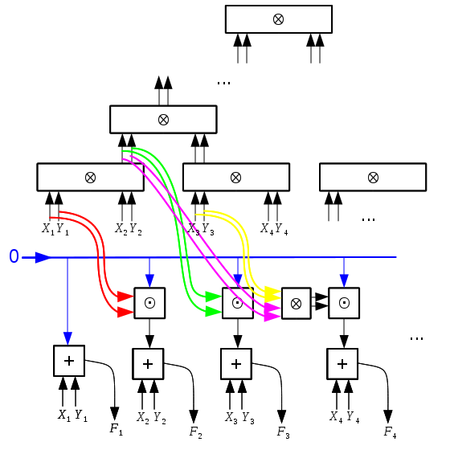
\includegraphics[height=9.1cm]{assets/summ.png}
\end{center}
Функции у конретной вершины в дереве будут такие:
\begin{enumerate}
    \item Получить от предка копозицию прошлых переполнений, которые не являются частью этого поддерева(если корень то получить k).
    \item Если вершина является листом, то передать полученную от предка композицию дальше в алгоритм, а предку вернуть значения переполнения этого бита.
    \item Передать левому ребенку композицию, полученную у предка, обратно получить композицию переполнения всего правого поддерева.
    \item Сделать композицию результата предка и левого сына и передать все это правому.
    \item Получить от правого композицию переполнений правого поддерева, сделать композицию предка, левого поддерева и правого поддерева и вернуть все это предку.
\end{enumerate}

Этот алгоритм насчитает все переполнения, а глубина у него $O(\log_2n)$, так как переполнения любого бита сначала будет только подниматься от листа до какой-то вершины, а потом опускаться обратно до какого-то листа, и пройдет путь не более $2\log_2n$.

Полученные переполнения мы по отдельности сложим с битами обычным битовым сумматором (считая k нулем, а g единицей), за $O(n)$ и получим сумму.
\subsection{Вычитатор}
Если мы вспомним формулу обратного числа в дополнении до 2, то она будет равна: $-y=\thicksim y+1$. Инверсию всех битов можно сделать заранее, за $O(n)$, добавить единицу можно не делая отдельное сложение с 1, если мы передадим на корень не k, а g, что и будет косвенно означать сложение с 1.

\subsection{Умножатор}
При умножении двух $n$ битных чисел получается $2n$ битное число, тогда для начала вспомним, как мы умножаем числа в столбик. При умножении чисел длины $n$ в столбик мы складываем $n$ чисел длины не более $2n$. Воспользуемся деревом Уоллеса для того, чтобы свести сумму $n$ чисел к сумме двух, которые мы уже честно сложим двоичным каскадным сумматором.
\subsubsection{Дерево Уоллеса}
Предположим, что у нас есть три числа, которые мы хотим сложить, длины не более $n$, сумма которых по длине также не превысит $n$, тогда мы можем разбить их на биты и каждый бит сложить битовым сумматором с переполнением. Полученные биты без переполнения будут объединены и станут первым числом, объединенные биты переполенения сдвинутые на 1 влево станут вторым числом. Эти 2 числа по сумме будут равным трем до, значит с помощью такой схемы мы за глубину 1 можем уменьшить количество элементов, которые нам надо сложить. 

\begin{center}
    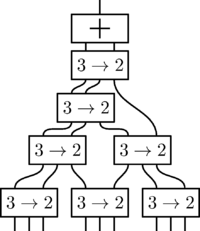
\includegraphics[height=9.1cm]{assets/wallace.png}
  \end{center}

